From the given info, 
% \begin{enumerate}
% Given the planes,
% \begin{align}
% P_1:\myvec{2&2&-3}\vec{x}&=5 \\
% P_2 :\myvec{3&-3&5} \vec{x}&=3
% \end{align}
The normal vectors of the given planes are 
\begin{equation}
 \vec n_1=\myvec{2\\2\\-3},
 \vec n_2 =\myvec{3\\-3\\5},
\end{equation}
%
Let $\theta$ be angle between vectors $\vec{n}_1$,$\vec{n}_2$.  Then,
\begin{align}
    \theta &= \cos^{-1}\brak{{\frac{\vec{n}_1^{T}\vec{n}_2}{\norm{\vec{n_1}}\norm{\vec{n}_2}}}}
 &=\cos^{-1}\brak{-\frac{1}{2}}\\
\implies \theta &= 120\degree
\end{align}
Fig.     \ref{linform/42/fig: PARALLEL planes.}  shows the two planes.
\begin{figure}[ht]
    \centering
   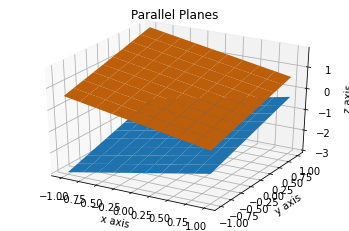
\includegraphics[width=\columnwidth]{solutions/su2021/2/42/Figure3.png}
    \caption{Parallel planes}
    \label{linform/42/fig: PARALLEL planes.}
\end{figure}    

  
 







